\chapter[Fundamentals of Electromagnetism][Fundamentals of Electromagnetism]{Fundamentals of Electromagnetism} \label{ch:Electromagnetism}
%
\section{Outline of Chapter}
%
In this chapter, I will cover the fundamental concepts from electromagnetism which will prove crucial for understanding this work. Starting from Maxwell's equations, I will derive the vector Helmholtz equation in the Fourier domain for linear isotropic media; the vector Helmholtz equation is the governing equation for this work. Next, I will derive a common model for the optical properties of dielectrics, the Lorentz model, and will discuss my work using reflection measurements to fit the Lorentz model for the polymer polydimethylsiloxane (PDMS).


\section{Maxwell's Equations} \label{sec:MaxwellEquations}
%
Maxwell's equations describe the origin and evolution of electric and magnetic fields, which are critical when determining radiative heat transfer. These fields can be created by charges, currents, or changes in the fields themselves. In the time domain, the macroscopic set of equations at position $\boldsymbol{r}$ and time $t$ are given by
\begin{subequations}
\begin{align}
\boldsymbol{\nabla} \cdot \widehat{\boldsymbol{D}}(\boldsymbol{r}, t) &= \widehat{\rho}_e(\boldsymbol{r}, t) \label{eq:ElectricDivergence}
\\
\boldsymbol{\nabla} \cdot \widehat{\boldsymbol{B}}(\boldsymbol{r}, t) &= \widehat{\rho}_m(\boldsymbol{r}, t) \label{eq:MagneticDivergence}
\\
\boldsymbol{\nabla} \times \widehat{\boldsymbol{E}}(\boldsymbol{r}, t) &= - \frac{\partial \widehat{\boldsymbol{B}}(\boldsymbol{r}, t)}{\partial t} - \widehat{\boldsymbol{J}}^m(\boldsymbol{r}, t) \label{eq:MaxwellCurlElectric1}
\\
\boldsymbol{\nabla} \times \widehat{\boldsymbol{H}}(\boldsymbol{r}, t) &= \frac{\partial \widehat{\boldsymbol{D}}(\boldsymbol{r}, t)}{\partial t} + \widehat{\boldsymbol{J}}^e(\boldsymbol{r}, t) \label{eq:MaxwellCurlMagnetic1}
\end{align}
\end{subequations}
%
where $\boldsymbol{\nabla} \cdot \left( \cdot \right)$ and $\boldsymbol{\nabla} \times \left( \cdot \right)$ denote the divergence and curl operators; $\widehat{\boldsymbol{D}}$, $\widehat{\boldsymbol{E}}$, $\widehat{\boldsymbol{B}}$, and $\widehat{\boldsymbol{H}}$ are the displacement, electric, magnetic flux density, and magnetic fields respectively; $\widehat{\rho}_e$ and $\widehat{\rho}_m$ are the electric and magnetic current densities; and $\widehat{\boldsymbol{J}}^e$ and $\widehat{\boldsymbol{J}}^m$ are the electric and magnetic free current densities. The hat over various symbols indicates the quantity is expressed in the time domain.

The version of Maxwell equations presented above has a number of magnetic terms added to the traditionally presented equations.\cite{Jackson1998} The terms are added to enforce symmetry between the electric and magnetic equations, but ultimately have little bearing on results, since the added terms can be set to zero later to recover the more traditional form of the equations. 

It will prove advantageous to work with Maxwell's equations in their time harmonic form, i.e. assume $\widehat{\boldsymbol{F}}(\boldsymbol{r}, t) = \mathrm{Re}[{\boldsymbol{F}}(\boldsymbol{r}) e^{-i \omega t}]$, where $\widehat{\boldsymbol{F}}$ can be $\widehat{\boldsymbol{D}}$, $\widehat{\boldsymbol{E}}$, $\widehat{\boldsymbol{B}}$, or $\widehat{\boldsymbol{H}}$, $\omega$ is the angular frequency, and $\mathrm{Re}(\cdot)$ indicates the real component of a complex number. Focusing now on Eqs. \ref {eq:MaxwellCurlElectric1} and \ref {eq:MaxwellCurlMagnetic1} and moving from the time domain to the Fourier domain, we get
%
\begin{subequations}
\begin{align}
\boldsymbol{\nabla} \times \boldsymbol{E}(\boldsymbol{r}) &= i \omega \boldsymbol{B}(\boldsymbol{r}) - \boldsymbol{J}^m(\boldsymbol{r}) \label{eq:MaxwellCurlElectric2}
\\
\boldsymbol{\nabla} \times \boldsymbol{H}(\boldsymbol{r}) &= - i \omega \boldsymbol{D}(\boldsymbol{r}) + \boldsymbol{J}^e(\boldsymbol{r}) \label{eq:MaxwellCurlMagnetic2}
\end{align}
\end{subequations}

In order to proceed, we will reduce the number of unknown fields in Maxwell's equations to two: $\boldsymbol{E}$ and $\boldsymbol{H}$. The displacement and magnetic flux density fields are given, by definition, as
%
\begin{subequations}
\begin{align}
\boldsymbol{D}(\boldsymbol{r}) &= \varepsilon_{0} \left( \boldsymbol{E} + \varepsilon_{0}^{-1} \boldsymbol{P} \right)
\\
\boldsymbol{B}(\boldsymbol{r}) &= \mu_{0} \left( \boldsymbol{H} + \boldsymbol{M} \right)
\end{align}
\end{subequations}
%
where $\boldsymbol{P}$ and $\boldsymbol{M}$ are the polarization and magnetization fields and $\varepsilon_{0}$ and $\mu_{0}$ are the permittivity and permeability of free space. The free space permittivity and permeability are constants which are related to the speed of light in vacuum, $c$, by $c = 1/\sqrt{\varepsilon_{0} \mu_{0}}$.

Rather annoyingly, at least in the my field, the polarization and magnetization fields lack the apparent symmetry that Maxwell's equations deserve. But all is not lost. In this work, I will work exclusively with linear, isotropic medium which have constitutive relations 
%
\begin{subequations}
\begin{align}
\varepsilon_{0}^{-1} \boldsymbol{P} &= \chi_{e} \boldsymbol{E} \label{eq:Polarization}
\\
\boldsymbol{M} &= \chi_{m} \boldsymbol{H}
\end{align}
\end{subequations}

Here, $\chi_{e}$ and $\chi_{m}$ are the electric and magnetic susceptibilities, which are themselves defined as
%
\begin{subequations}
\begin{align}
\chi_{e} &= \varepsilon - 1 \label{eq:ElectricSusceptibility}
\\
\chi_{m} &= \mu - 1
\end{align}
\end{subequations}
%
in linear media. $\varepsilon$ and $\mu$ are the relative permittivity and permeability, respectively. $\varepsilon$ and $\mu$ are often written with an $r$ subscript (to indicate relative) in other works. The unsubscripted variables are then commonly used to denote the products of the relative and free space variables. But in this work, because we will rarely need the product of the relative and free space variables, that quantity will be given no symbol, and the other quantities will be defined as described above. $\varepsilon$ is also commonly called the dielectric function, and is explored thoroughly in Section \ref{sec:OpticalProperties}.

Now that all the groundwork has been laid, we can simplify Eqs. \ref{eq:MaxwellCurlElectric2} and \ref{eq:MaxwellCurlMagnetic2} to include only the electric and magnetic fields. The simplification yields
%
\begin{subequations}
\begin{align}
\boldsymbol{\nabla} \times \boldsymbol{E}(\boldsymbol{r}) &= i \omega \mu \mu_{0} \boldsymbol{H}(\boldsymbol{r}) - \boldsymbol{J}^m(\boldsymbol{r}) \label{eq:MaxwellCurlElectric3}
\\
\boldsymbol{\nabla} \times \boldsymbol{H}(\boldsymbol{r}) &= - i \omega \varepsilon \varepsilon_{0} \boldsymbol{E}(\boldsymbol{r}) + \boldsymbol{J}^e(\boldsymbol{r}) \label{eq:MaxwellCurlMagnetic3}
\end{align}
\end{subequations}

Finally, we can substitute Eqs. \ref{eq:MaxwellCurlElectric3} and \ref{eq:MaxwellCurlMagnetic3} into one another to achieve
\begin{subequations}
\begin{align}
\boldsymbol{\nabla} \times \boldsymbol{\nabla} \times \boldsymbol{H}(\boldsymbol{r}) - k^{2} \boldsymbol{H}(\boldsymbol{r}) &= i \omega \varepsilon \varepsilon_{0} \boldsymbol{J}^m(\boldsymbol{r}) + \boldsymbol{\nabla} \times  \boldsymbol{J}^e(\boldsymbol{r}) \label{eq:MaxwellCurlElectric4}
\\
\boldsymbol{\nabla} \times \boldsymbol{\nabla} \times \boldsymbol{E}(\boldsymbol{r}) - k^{2} \boldsymbol{E}(\boldsymbol{r})&= i \omega \mu \mu_{0} \boldsymbol{J}^e(\boldsymbol{r}) - \boldsymbol{\nabla} \times \boldsymbol{J}^m(\boldsymbol{r}) \label{eq:MaxwellCurlMagnetic4}
\end{align}
\end{subequations}
%
where $k = (\omega/c) \sqrt{\varepsilon \mu}$ is the wavevector. Eqs. \ref{eq:MaxwellCurlElectric4} and \ref{eq:MaxwellCurlMagnetic4} are examples of the inhomogeneous vector Helmholtz equation. The challenge now is to invert the equations to obtain $\boldsymbol{E}$ and $\boldsymbol{H}$. This can be achieved using dyadic Green's functions, which will be discussed in Chapter \ref{ch:DGFs}.


\section{Optical Properties of Materials} \label{sec:OpticalProperties}

\subsection{Overview}
%
When discussing the optical properties of linear isotropic media, there are three crucial unitless parameters: the dielectric function, relative permeability, and refractive index. In general, all three quantities are complex-valued and frequency-dependent. The dielectric function (relative permeability) is a measure of a material's degree of polarization (magnetization) under the influence of an externally applied electric (magnetic) field. The refractive index describes how light propagates through a medium. Its real and imaginary parts correspond to speed and dissipation of light as it passes through the medium, respectively. The three quantities are related to one another by
%
\begin{equation}
n_{c} = \sqrt{\varepsilon \mu} = n + i \kappa
\end{equation}
%
where $n_{c}$ is the complex refractive index and $n$ and $\kappa$ are the real and imaginary components of $n_{c}$. $n$ is the refractive index and $\kappa$ is the extinction coefficient. In the infrared portion of the electromagnetic spectrum where this work is focused, most materials do not exhibit magnetic behavior ($\mu \approx 1$). Thus, the subsequent discussion in this section will focus on the dielectric function. 


\subsection{Dielectric Function}
%
\begin{figure}
\centering
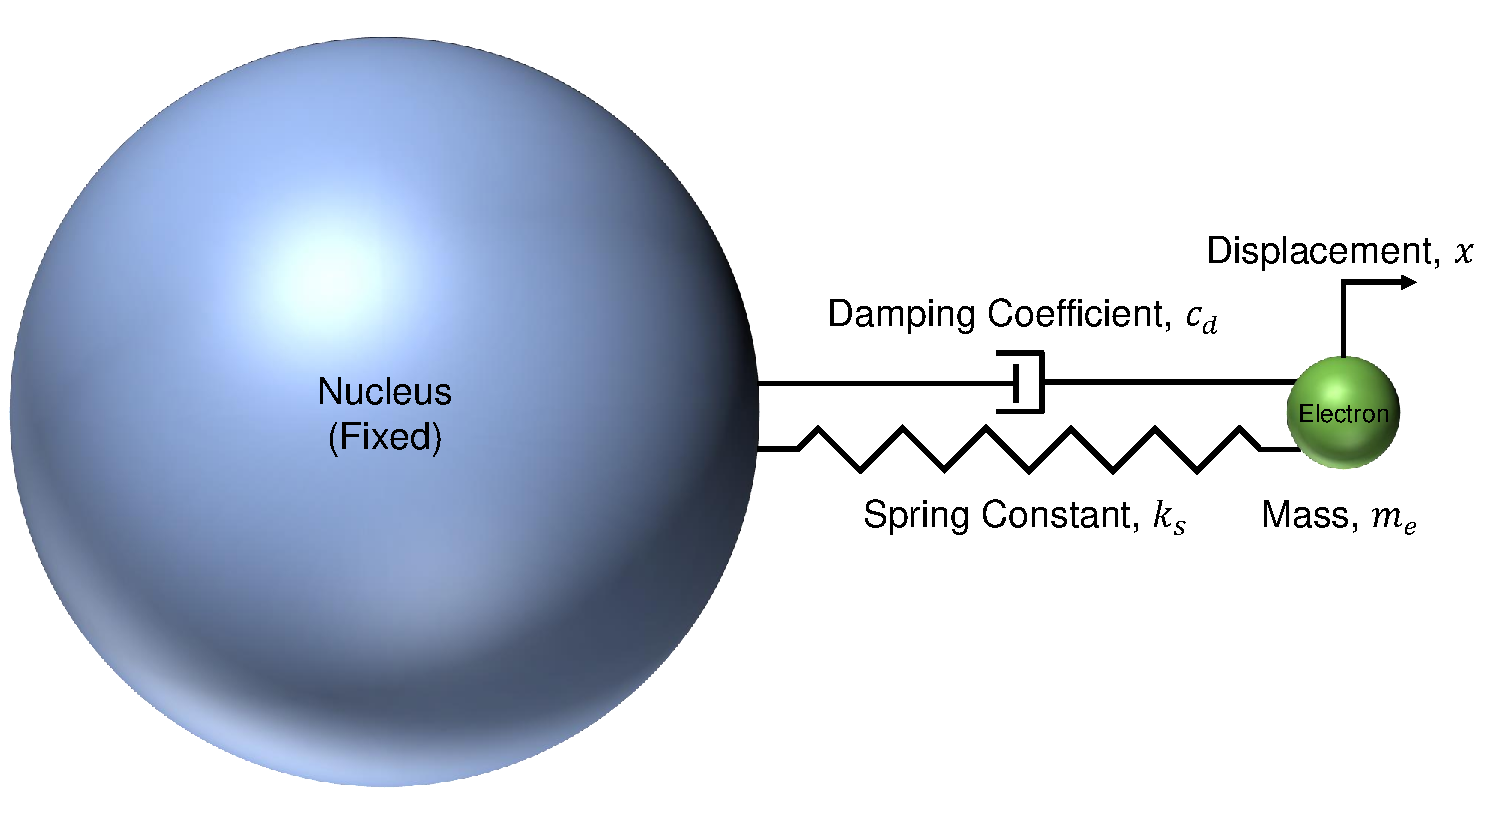
\includegraphics[width=0.8\textwidth]{./Figures/SpringMassDamper.pdf}
\caption{\label{fig:SpringMassDamper}Conceptual diagram of the spring-mass-damper system of an electron bound to its nucleus.}
\end{figure}
%
To derive a model for the dielectric function, we will examine the dynamics of a bound electron around a nucleus, which can be approximated by a spring-mass-damper system (see Fig. \ref{fig:SpringMassDamper}). In the time domain, the governing equation of such a system is
%
\begin{equation}
\widehat{\boldsymbol{F}} = m_{e} \ddot{\widehat{\boldsymbol{x}}} + c_{d} \dot{\widehat{\boldsymbol{x}}} + k_{s} \widehat{\boldsymbol{x}}
\end{equation}
%
where a dot indicates a time derivative. Again assuming a time harmonic response and moving into the Fourier domain, the equivalent equation is
%
\begin{equation}
\boldsymbol{F} = \left( - \omega^{2} m_{e} - i \omega c_{d} + k_{s} \right) \boldsymbol{x}
\end{equation}

Further simplification can be made by using insight from spring-mass damper systems. The undamped resonant frequency and damping factor, $\omega_{0}$ and $\zeta$, are defined as $\omega_{0} = \sqrt{k_{s}/m_{e}}$ and $\zeta = c_{d}/(2\sqrt{k_{s}m_{e}})$, respectively. Substituting in accordingly, we get
%
\begin{equation}
\boldsymbol{F} = m_{e} \left( - \omega^{2} - i2 \omega \omega_{0} \zeta + \omega_{0}^{2} \right) \boldsymbol{x}
\end{equation}

Next, we must use insight from electromagnetism. First, the force on a particle in a uniform electric field is $\boldsymbol{F} = q_{e} \boldsymbol{E}$, where $q_{e}$ is the charge of the particle. Further, the polarization field is related to the displacement by $\boldsymbol{P} = N_{e} q_{e} \boldsymbol{x}$, where $N_{e}$ is the average number of electrons in a unit volume. These facts, in conjunction with Eqs. \ref{eq:Polarization} and \ref{eq:ElectricSusceptibility}, yield
%
\begin{equation}
\boldsymbol{x} = \frac{\varepsilon_{0} \left( \varepsilon - 1 \right)}{N q_{e}} \boldsymbol{E}
\end{equation}

Putting everything together and solving for $\varepsilon$, we arrive at
%
\begin{equation}
\varepsilon = 1 + \frac{S}{1 - \left( \frac{\omega}{\omega_{0}} \right)^{2} - i \Gamma \left( \frac{\omega}{\omega_{0}} \right)}
\end{equation}
%
where $\Gamma = 2 \zeta$ and $S = N_{e} q_{e}^{2} / (w_{0}^{2} m_{e} \varepsilon_{0})$. This derived model is the simplest form of the Lorentz oscillator model. In reality, not all materials are composed of only identical nuclei and bound electrons like Fig. \ref{fig:SpringMassDamper} depicts. Many common dielectrics are composed of atoms arranged with multiple covalent bonds, each with its own resonant frequency. Thus, its is not unreasonable to expect that such a material's dielectric function would reflect the multiple resonances. These multiple resonances are accounted for by summing over the necessary number of oscillators
%
\begin{equation}
\varepsilon = \varepsilon_{\infty} + \sum_{j=1}^{N_{\mathrm{max}}} \left[ \frac{S_{j}}{1 - \left( \frac{\omega}{\omega_{0,j}} \right)^{2} - i \Gamma_{j} \left( \frac{\omega}{\omega_{0,j}} \right)} \right]
\end{equation}

The constant value of 1 was replaced by $\varepsilon_{\infty}$ because researchers often look at only a portion of the electromagnetic spectrum. Any oscillators with resonant frequencies much higher than the portion of the spectrum being examined manifest as an additional offset. For example, the parameters of a Lorentz model for polymethylmethacrylate (PMMA) are shown in Table. \ref{tab:PMMALorentzModel}. The Lorentz oscillator model is just one among many models for the dielectric function. Other common models are listed in Table \ref{tab:DielectricFunctionModels}.

\begin{table}
	\caption{\label{tab:PMMALorentzModel} Oscillator parameters determined to reproduce the dielectric function of PMMA.\cite{Tsuda2018} Unlisted is $\epsilon_{\infty}$ = $2.162$.}
	\begin{center}
		\renewcommand{\arraystretch}{1.15}
		\setlength{\tabcolsep}{0.10cm}
		\begin{tabular}{llllllllll}
			\hline 
			\hline
			\multicolumn{1}{c}{$j$} &
			\multicolumn{1}{c}{$\hbar \omega_{0}$ (eV)} & \multicolumn{1}{c}{$\lambda_{0}$ (\si{\micro\meter})} &
			\multicolumn{1}{c}{$S$} &
			\multicolumn{1}{c}{$\Gamma$} &
			\multicolumn{1}{c}{$j$} &
			\multicolumn{1}{c}{$\hbar \omega_{0}$ (eV)} & \multicolumn{1}{c}{$\lambda_{0}$ (\si{\micro\meter})} &
			\multicolumn{1}{c}{$S$} &
			\multicolumn{1}{c}{$\Gamma$} \\ 	
			\hline 
			%
			1 & 0.09327 & 13.29 & 3.18$ \times 10^{-3}$ & 0.01815 & 13 & 0.1688 & 7.345 & 1.09$ \times 10^{-3}$ & 0.03083 \\
			2 & 0.1002 & 12.37 & 6.94$ \times 10^{-4}$ & 0.01919 & 14 & 0.1720 & 7.207 & 1.07$ \times 10^{-3}$ & 0.01139 \\
			3 & 0.1023 & 12.12 & 1.13$ \times 10^{-4}$ & 0.005102 & 15 & 0.1779 & 6.970 & 1.34$ \times 10^{-3}$ & 0.007360 \\
			4 & 0.1045 & 11.86 & 2.86$ \times 10^{-3}$ & 0.02739 & 16 & 0.1799 & 6.894 & 4.11$ \times 10^{-3}$ & 0.01734 \\
			5 & 0.1133 & 10.94 & 1.68$ \times 10^{-3}$ & 0.03556 & 17 & 0.1837 & 6.748 & 2.12$ \times 10^{-3}$ & 0.01294 \\
			6 & 0.1197 & 10.36 & 3.94$ \times 10^{-3}$ & 0.02766 & 18 & 0.2145 & 5.7780 & 1.56$ \times 10^{-2}$ & 0.005433 \\
			7 & 0.1227 & 10.11 & 2.79$ \times 10^{-3}$ & 0.01483 & 19 & 0.3522 & 3.520 & 6.66$ \times 10^{-5}$ & 0.005393 \\
			8 & 0.1322 & 9.38 & 1.10$ \times 10^{-3}$ & 0.01272 & 20 & 0.3621 & 3.424 & 8.42$ \times 10^{-4}$ & 0.02086 \\
			9 & 0.1425 & 8.700 & 2.92$ \times 10^{-2}$ & 0.02708 & 21 & 0.3658 & 3.389 & 6.60$ \times 10^{-4}$ & 0.006372 \\
			10 & 0.1476 & 8.401 & 1.04$ \times 10^{-2}$ & 0.01858 & 22 & 0.3717 & 3.336 & 9.53$ \times 10^{-4}$ & 0.01224 \\
			11 & 0.1539 & 8.056 & 6.64$ \times 10^{-3}$ & 0.01722 & 23 & 0.4265 & 2.907 & 4.15$ \times 10^{-5}$ & 0.009852 \\
			12 & 0.1574 & 7.877 & 5.49$ \times 10^{-3}$ & 0.01942 &  &  &  &  &  \\
			\hline
			\hline
		\end{tabular} 
	\end{center}
\end{table}

\begin{table}
	\caption{\label{tab:DielectricFunctionModels}Common dielectric function models, presented in terms of angular frequency. $A$, $S$, $\omega_{0}$, $\Gamma$, $\varepsilon_{\infty}$, and $\omega_{p}$ are model parameters that must be determined for a given material.}
	\begin{center}
		\renewcommand{\arraystretch}{1.15}
		\setlength{\tabcolsep}{0.10cm}
		\begin{tabular}{llllllll}
			\hline 
			\multicolumn{1}{c}{Name} &
			\multicolumn{1}{c}{Model} & 
			\multicolumn{1}{c}{Applicability} \\
			\hline
			%
			Cauchy & $\varepsilon(\omega) = \left[ \sum_{j=0}^{N_{\mathrm{max}}} A_{j} \omega^{2j} \right]^{2}$ & Glassy Dielectrics \\
			Sellmeier & $\varepsilon(\omega) = \varepsilon_\infty + \sum_{j=1}^{N_{\mathrm{max}}} \left[ \frac{S_{j} }{1 - ( \omega / \omega_{0,j} )^{2} } \right]$ & Glassy Dielectrics \\
			Lorentz & $\varepsilon(\omega) = \varepsilon_\infty + \sum_{j=1}^{N_{\mathrm{max}}} \left[ \frac{S_{j} }{1 - ( \omega / \omega_{0,j} )^{2} -  i \Gamma_{j} (\omega / \omega_{0,j} ) } \right]$ & Crystalline Dielectrics \\
			Brendel-Bormann & See Ref. \citenum{Brendel1992}. & Amorphous Dielectrics \\
			Causal Voigt & See Ref. \citenum{DeSousaMeneses2005}. & Amorphous Dielectrics \\
			Drude & $\varepsilon(\omega) = 1 - \frac{\omega_p^2}{\left( \omega^2 +  i \Gamma \omega \right)}$ & Metals \\
			\hline
		\end{tabular} 
	\end{center}
\end{table}


\subsection{Method of Determining Dielectric Function}
%
Several methods of determining the dielectric function of a material exist in the literature, including as refractometry,\cite{Burnett2016} ellipsometry,\cite{Jellison1993} and reflectometry using Kramers-Kronig analysis.\cite{Roessler1965, Roessler1965a} In this section, I will explain my work, performed by Srinivasan, Czapla, Mayo, and Narayanaswamy (henceforth Srinivasan et al.), which focused on extracting the dielectric function of polydimethylsiloxane (PDMS) from reflection measurements by fitting a Lorentz model.\cite{Srinivasan2016} PDMS is a silicone elastomer which has a diverse set of applications ranging from MEMS\cite{Streque2010} and microfluidic devices\cite{Fujii2002, Lamberti2015, You2015} to surfactant\cite{Laubie2013} and antifoamer technologies.\cite{Owen2012}  It is well-known that PDMS is highly transmissive between 0.4 \si{\micro\meter} and 1.8 \si{\micro\meter}, making it attractive for optical waveguide communication and optofluidic applications.\cite{Mata2005, Psaltis2006, Cai2008, Cai2010, Cai2013} At the time Ref. \citenum{Srinivasan2016} was published, the complex refractive index of the solid form of PDMS had previously been reported only for visible to near-infrared wavelengths\cite{Spaeth1997, Cardenas-Valencia2006, Kopetz2007, Schneider2009, Cai2010, Cai2013, Kacik2014} and for wavelengths in the far-infrared or longer.\cite{Podzorov2008, Wang2012a, Khodasevych2012, Headland2015} A liquid form of PDMS was investigated by Querry in the range from 0.8 \si{\micro\meter} to 55.6 \si{\micro\meter}.\cite{Querry1987} Since the publication of Ref. \citenum{Srinivasan2016}, Motaharifar et al. also examined the infrared optical properties of PDMS.\cite{Motaharifar2018}

\begin{figure}
\centering
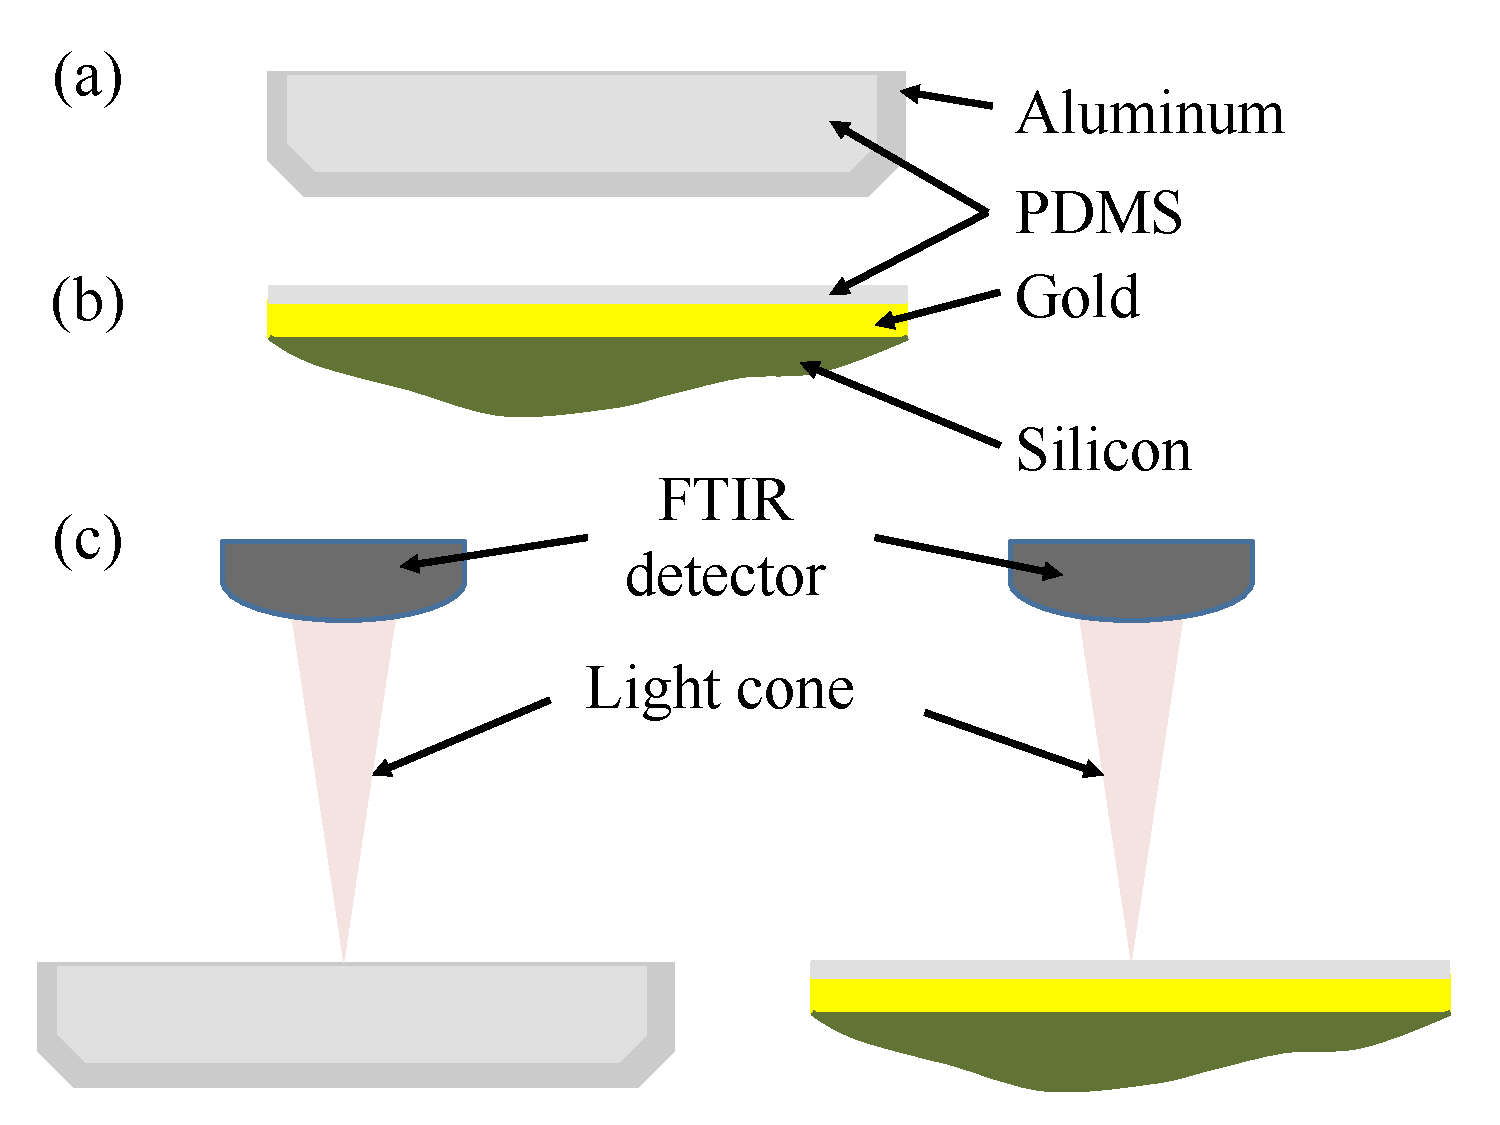
\includegraphics[width=0.8\textwidth]{./Figures/PDMS_Geometry.pdf}
\caption{\label{fig:PDMS_Geometry}(a) Geometry of bulk PDMS samples prepared in aluminum dishes. (b) PDMS thin film on top of gold coated silicon substrate. (c) Normal incidence FTIR spectroscopy reflectance measurements.}
\end{figure}

Srinivasan et al. determined the complex refractive index of PDMS between 2.5 \si{\micro\meter} and 16.7 \si{\micro\meter} by fitting a Lorentz model to Fourier transform infrared (FTIR) reflectance measurements made on bulk PDMS and thin films of PDMS deposited on gold coated silicon substrates. Henceforth, I will refer to these PDMS thin films atop gold coated substrates as simply PDMS thin films. PDMS polymer was prepared from a Sylgard\textsuperscript{\textregistered} 184 elastomer kit with a base to curing agent mass ratio of 10:1. The solution was then de-gassed under low vacuum for an hour and poured into aluminum dishes as shown in Fig. \ref{fig:PDMS_Geometry}(a).  The samples were subsequently cured in a furnace at 75\si{\celsius} for at least 1.5 hours and were approximately 8 \si{\milli \meter} thick. FTIR transmittance measurements made on 8 \si{\milli \meter} samples showed an average transmittance of 0.2\%, confirming that they may be treated as bulk.

To create PDMS thin films, 50 \si{\nano\meter} of gold was deposited on silicon wafers using an Edwards 306\textsuperscript{\textregistered} Thermal Evaporator. This configuration is shown in Fig. \ref{fig:PDMS_Geometry}(b). The high value of $\kappa$ for gold ensures that 50 \si{\nano\meter} is sufficiently thick to suppress any potential backside reflections and to be treated as optically bulk.\cite{Ordal1985} PDMS was spin coated on top of the gold layer using a Laurel WS-650Sz-6NPP-Lite\textsuperscript{\textregistered} spinner. The thin film PDMS samples were then cured at 75\si{\celsius} for 1 hour. The spin rates and duration were adjusted to achieve films of different thicknesses. A Filmetrics F20\textsuperscript{\textregistered} instrument, which uses a spectral reflectance technique at normal incidence in the wavelength range of 0.2 \si{\micro\meter} to 1.1 \si{\micro\meter} was used to measure the thickness of PDMS thin films. The Sellmeier dispersion model for the refractive index of PDMS in this wavelength range\cite{Schneider2009} was used to calculate the thickness based on goodness-of-fit between calculated and measured reflectance spectra. Table \ref{tab:Filmthick} shows the mean and standard deviation of thickness measurements. The values are based on at least three measurements taken at different locations on each sample. The variation in thickness values between locations is due to non-uniformity of the PDMS surface caused by factors such as eccentricity of the initial PDMS droplet on the wafer, rate of shrinkage of PDMS after spin-coating, and dynamics of the spin coating motor.\cite{Krishnan2007}

\begin{table}
	\caption{\label{tab:Filmthick} Measurements of film thickness for PDMS thin film samples}
	\begin{center}
		%		\renewcommand{\arraystretch}{1.3 }
		%		\setlength{\tabcolsep}{0.1cm}
		%\newcolumntype{L}{>{\centering\arraybackslash}m{3cm}}
		\begin{tabular}{ccc}
			\hline 
			\hline
			\multicolumn{1}{c}{Thin Film (TF)} & \multicolumn{1}{c}{Mean (\si{\micro\meter})} & \multicolumn{1}{c}{Standard Deviation (\si{\micro\meter})} \\
			\hline 
			
			TF1 &     11.7   & $2.51\times 10^{-1}$ \\ 
			%			2 &     11.7   & $0.435\times 10^{-1}$ \\ 
			TF2 &     7.43   & $1.25\times 10^{-1}$ \\ 
			%			4 &     7.53   & $1.85\times 10^{-1}$ \\ 
			
			\hline
			\hline
		\end{tabular} 
	\end{center}
\end{table}

Reflectance spectra were measured using a Bruker Hyperion FTIR microscope with a 15x, 0.4 numerical aperture objective at normal incidence to the PDMS samples. The measurements were taken in reflection mode (reflected intensity from the sample is  normalized by the reflected intensity from clean gold) at 64 scans per recording. Srinivasan et al. measured 50 reflectance spectra on 3 different locations for both bulk PDMS and PDMS thin film samples.

Following the procedure outlined by Verleur,\cite{Verleur1968} Srinivasan et al. extracted the optical properties of PDMS by fitting the FTIR reflectance measurements to simulated reflectance curves. The simulated curves were calculated using a Lorentz oscillator model for the dielectric function of PDMS with an initial set of assumed trial parameters (i.e. $\omega_{0}$, $S$, $\Gamma$, and $\varepsilon_{\infty}$). The relative permeability was assumed to be unity, because PDMS is non-magnetic. Fresnel coefficients were then used to compute the theoretical reflectance for samples with the trial parameters. The normal incidence reflectance, $R_{calc}(\omega)$, is given by
%
\begin{equation}
R_{calc}(\omega) =
\left\{\begin{array}{lll}
\left| r_{12}(\omega) \right|^{2} & \text{for bulk samples} \\
\left| \frac{ r_{12} + r_{23} \exp{\left( 2i k_{2} d_{2} \right)} }{ 1 + r_{12} r_{23} \exp{\left( 2i k_{2} d_{2} \right)} } \right|^{2} & \text{for thin film samples}
\end{array} \right.
\end{equation}
%
where $r_{ij}$ is the Fresnel reflection coefficient (for either s or p polarization) at normal incidence at the interface between materials $i$ and $j$. A full description of the Fresnel coefficients can be found in Appendix \ref{ap:FresnelCoefficients}. In this case, materials 1, 2, and 3 are vacuum, PDMS, and gold respectively and $d_{2}$ is the thickness of the PDMS thin film. Srinivasan et al. used the complex refractive index for gold obtained from Ordal et al.\cite{Ordal1985}

A constrained nonlinear optimization function called \textit{fmincon} in MATLAB\textsuperscript{\textregistered} was used to fit the measured reflectance curves and produce a final set of dielectric function parameters from the set of trial parameters. The fitting algorithm minimized the value of error given by
%
\begin{equation}
\label{eqn:fsse}
e = \sum_{j=1}^{N_{\text{meas}}} \sum_{i=1}^{N_{\omega}} w_{j} \left[ R_{\text{meas},j}(\omega_{i}) - R_{\text{calc},j}(\omega_{i}) \right]^2
\end{equation}
%
where $N_{\mathrm{meas}}$ is total the number of measured FTIR reflectance spectra (including bulk and thin film measurements); $N_{\omega}$ is the number of frequency points in a measured reflectance spectrum;  $R_{\text{meas},j}(\omega_{i})$ and $R_{\text{calc},j}(\omega_{i})$ are the reflectance at $\omega_{i}$ in the $j^{\text{th}}$ measurement and $j^{\text{th}}$ calculation, respectively; and $w_{j}$ is a weight function.

Initially, Srinivasan et al. extracted the parameters of the Lorentz oscillator model by fitting the reflectance measurements of the bulk sample alone. On noticing that the extracted parameters could not accurately reproduce some features of the reflectance spectra from thin films, Srinivasan et al. decided to include both bulk and thin film reflectance spectra in our measure of error. 

In order to account for the difference in magnitude between the bulk and thin film reflectances, the weight function, $w_j$, was introduced. For bulk reflectance spectra, $w_{j} = 25$ and for thin films reflectance spectra, $w_{j} = 1$. The choice of $w_j$ for bulk and thin film samples was made based on the maximum reflectance in each case.

\begin{table}
	\caption{\label{tab:MinParam} Oscillator parameters determined to reproduce the dielectric function of PDMS. Unlisted is $\epsilon_{\infty}$ = $2.276$.}
	\begin{center}
		\renewcommand{\arraystretch}{1.15}
		\setlength{\tabcolsep}{0.10cm}
		\begin{tabular}{ccccccccc}
			\hline 
			\hline
			\multicolumn{1}{c}{$j$} &
			\multicolumn{1}{c}{$\hbar \omega_{0}$ (eV)} &  \multicolumn{1}{c}{$S$} &
			\multicolumn{1}{c}{$\Gamma$} &
			\multicolumn{1}{c}{$j$} &
			\multicolumn{1}{c}{$\hbar \omega_{0}$ (eV)} &  \multicolumn{1}{c}{$S$} &
			\multicolumn{1}{c}{$\Gamma$} \\ 	
			\hline 
			%
			1 & $0.0737$ & $0.0021$ & $0.0211$ &   9 & $0.1279$ & $0.0288$ & $0.0152$ \\
			2 & $0.0821$ & $0.0029$ & $0.0146$ & 10 & $0.1343$ & $0.1181$ & $0.0376$ \\
			3 & $0.0846$ & $0.0090$ & $0.0307$ & 11 & $0.1561$ & $0.0087$ & $0.0061$ \\ 
			4 & $0.0870$ & $0.0142$ & $0.0453$ & 12 & $0.1749$ & $0.0005$ & $0.0102$ \\
			5 & $0.0938$ & $0.0021$ & $0.0097$ & 13 & $0.1798$ & $0.0005$ & $0.0252$ \\
			6 & $0.0994$ & $0.0913$ & $0.0238$ & 14 & $0.3631$ & $0.0006$ & $0.0525$ \\
			7 & $0.1046$ & $0.0175$ & $0.0184$ & 15 & $0.3672$ & $0.0006$ & $0.0050$ \\
			8 & $0.1077$ & $0.0121$ & $0.0137$ &  &  &  & \\
			\hline
			\hline
		\end{tabular} 
	\end{center}
\end{table}

Srinivasan et al. empirically determined that using a set of 15 oscillators produced the best fit. To account for the sensitivity of final parameters to  the initial trial parameters, 5000 sets of trial parameters were created by randomly varying their values by $1 \%$ for resonant frequency and $5 \%$ for all remaining parameters. The set of oscillator parameters that yielded the lowest total error (Eq. \ref{eqn:fsse}) is provided in Table \ref{tab:MinParam}. As discussed by Verleur,\cite{Verleur1968} one or more oscillators outside the frequency range of the measurement spectrum may be needed to produce an accurate fit. The optimization routine placed a single oscillator located at $0.0737$ eV (16.8 \si{\micro\meter}) with appropriate strength and damping values to minimize the error. This however, does not imply that the fit is valid outside the measured 2.5 \si{\micro\meter} to 16.7 \si{\micro\meter} range.

Figure \ref{fig:RelectanceError} shows the measured and fitted reflectance spectra. The gray shaded bands in Fig. \ref{fig:RelectanceError} are composed of spectra from the 5000 sets of final parameters. The spectra from the set of oscillator parameters that yielded the lowest total error over all bulk and thin film measurements is also shown as the solid line in Fig. \ref{fig:RelectanceError}.

The real and imaginary parts of the complex refractive index are shown in Fig. \ref{fig:RefInd}. The higher values of extinction coefficient beyond $8$ $\mu$m correspond to high absorption bands.\cite{Cai2010} Interestingly, these strong absorption bands show PDMS has the potential to act as a passive radiative cooling device.\cite{Czapla2017a}

\begin{figure}
\centering
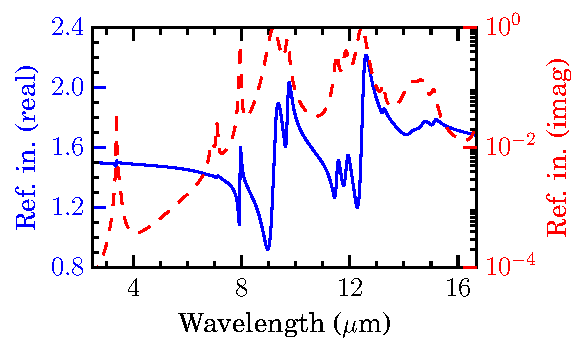
\includegraphics[width=0.8\textwidth]{./Figures/PDMS_RefractiveIndex.pdf}
\caption{\label{fig:RefInd}Real ($n$, solid line, left y-axis) and imaginary ($\kappa$, dashed line, right y-axis) parts of the complex refractive index of PDMS, respectively.}
\end{figure}

\begin{figure}
\centering
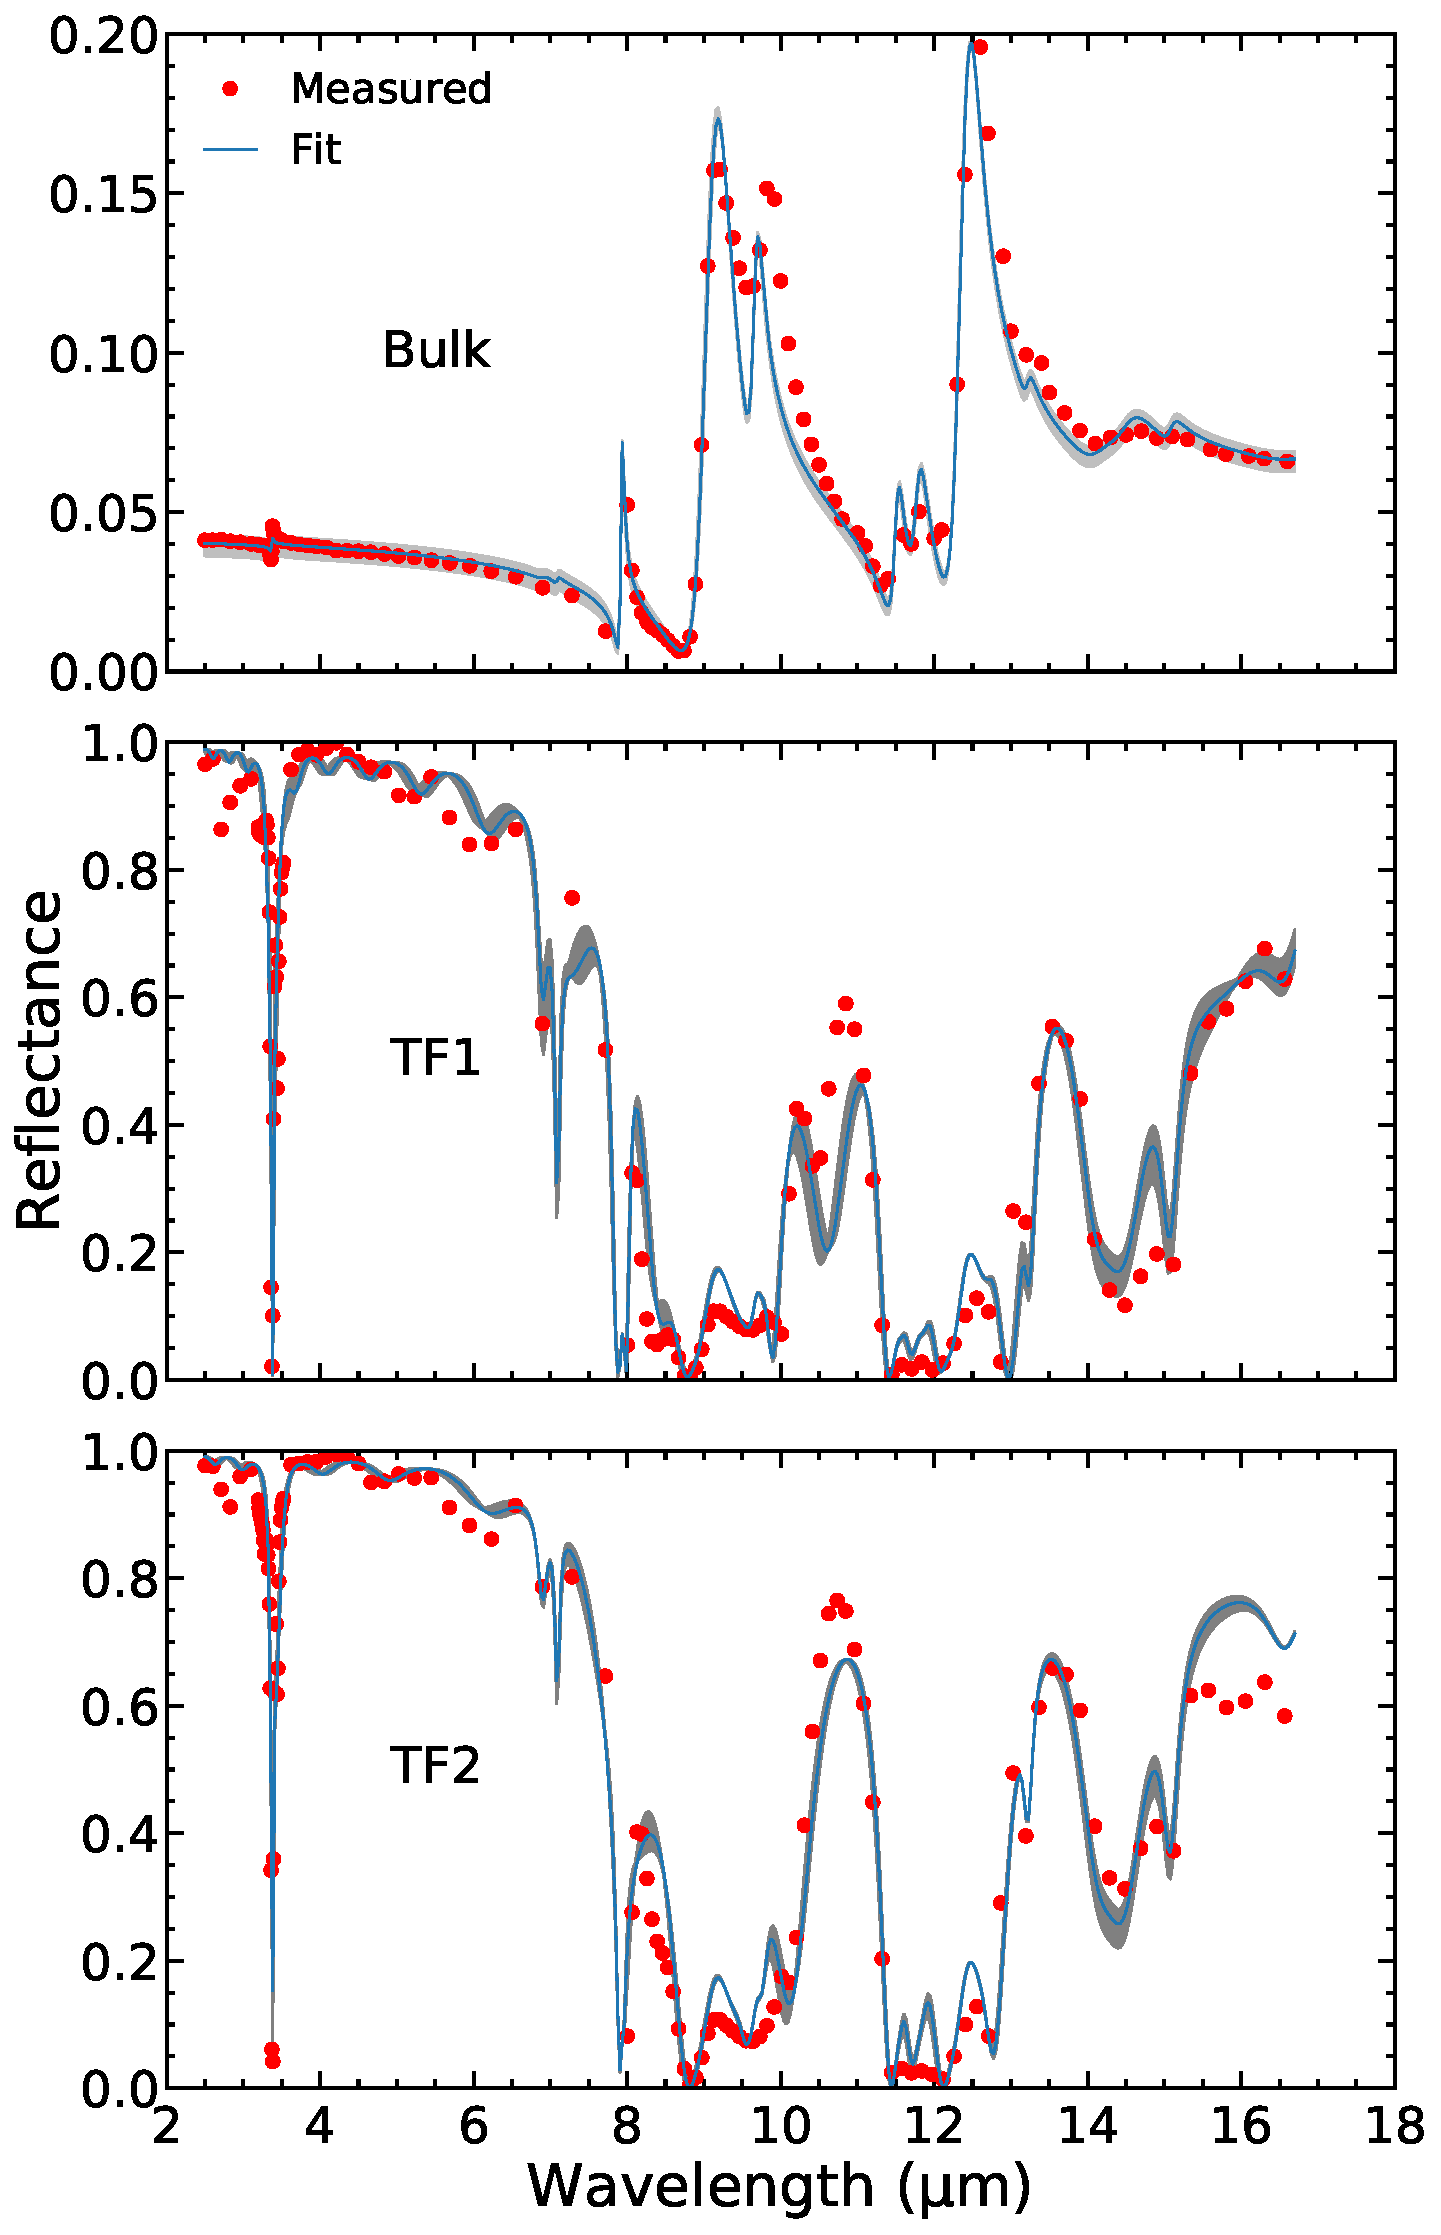
\includegraphics[width=0.75\textwidth]{./Figures/PDMS_Reflectance_and_Fit.pdf}
\caption{\label{fig:RelectanceError} Reflectance spectra of bulk and thin film PDMS samples at normal incidence obtained from FTIR reflectance measurements (circular markers); all 5000 sets of extracted oscillator parameters (gray shaded band); and the set of oscillator parameters with the lowest total error over all measurements (solid line). For clarity, only a representative number of measurement data points (circular markers) are shown.}
\end{figure}





